\documentclass[10pt,a4paper]{extarticle}
\usepackage[top=1.9cm,bottom=1.9cm,left=1.9cm,right=1.9cm,headheight=15pt]{geometry}
\usepackage{fontspec}
\usepackage{polyglossia}
\setmainlanguage{russian}\setotherlanguage{english}
\setmainfont{Cambria}
\setsansfont{Calibri}
\setmonofont{Consolas}[Scale=0.88]
\usepackage{amsmath}
\usepackage{unicode-math}
\setmathfont{Cambria Math}
\usepackage[most]{tcolorbox}
\usepackage{fvextra}
\usepackage{graphicx}
\usepackage{booktabs,array,tabularx,multirow,colortbl}
\usepackage{xcolor}
\usepackage{tikz}
\usetikzlibrary{arrows.meta,positioning,shapes.geometric,calc,fit,backgrounds,decorations.pathreplacing}
\usepackage{enumitem}
\usepackage{titlesec}
\usepackage{microtype}
\usepackage{fancyhdr}
\usepackage{caption}
\usepackage{float}
\usepackage{needspace}
\usepackage{etoolbox}
\usepackage[hidelinks]{hyperref}

\definecolor{acc}{HTML}{1F4E79}
\definecolor{accL}{HTML}{DCE9F7}
\definecolor{accD}{HTML}{143552}
\definecolor{dataC}{HTML}{2E7D32}
\definecolor{dataL}{HTML}{DDEFDC}
\definecolor{parC}{HTML}{B45F06}
\definecolor{parL}{HTML}{FCE8D0}
\definecolor{badC}{HTML}{B3261E}
\definecolor{badL}{HTML}{F8DAD7}
\definecolor{goodC}{HTML}{2E7D32}
\definecolor{goodL}{HTML}{DDEFDC}
\definecolor{warnC}{HTML}{9A6700}
\definecolor{warnL}{HTML}{FFF4D1}
\definecolor{inkL}{HTML}{F4F6F8}
\definecolor{rule}{HTML}{C9D3DD}
\definecolor{tBg}{HTML}{16202B}
\definecolor{tBar}{HTML}{263445}
\definecolor{tText}{HTML}{D6DEE7}
\definecolor{tPrompt}{HTML}{F2C14E}
\definecolor{tCmd}{HTML}{FFFFFF}
\definecolor{tGood}{HTML}{6FD68A}
\definecolor{tBad}{HTML}{FF7B72}
\definecolor{tVerb}{HTML}{79C0FF}
\definecolor{tData}{HTML}{8EE3A4}
\definecolor{tParity}{HTML}{F6B26B}

\titleformat{\section}{\sffamily\Large\bfseries\color{acc}}{\thesection}{0.6em}{}[\vspace{-5pt}{\color{rule}\titlerule[0.8pt]}]
\titlespacing*{\section}{0pt}{16pt}{8pt}
\titleformat{\subsection}{\sffamily\large\bfseries\color{accD}}{\thesubsection}{0.5em}{}
\titlespacing*{\subsection}{0pt}{11pt}{4pt}
\titleformat{\subsubsection}{\sffamily\normalsize\bfseries\color{acc}}{}{0pt}{}
\titlespacing*{\subsubsection}{0pt}{7pt}{2pt}

\setlength{\parindent}{0pt}
\emergencystretch=3em
\tolerance=1500
\setlength{\parskip}{4pt}
\linespread{1.06}
\captionsetup{font={small,sf},labelfont={bf,color=acc},labelsep=period,skip=4pt}
\setlist[itemize]{leftmargin=5mm,itemsep=1.5pt,topsep=2pt,parsep=0pt}
\setlist[enumerate]{leftmargin=6mm,itemsep=1.5pt,topsep=2pt,parsep=0pt}

\pagestyle{fancy}\fancyhf{}
\renewcommand{\headrulewidth}{0.4pt}\renewcommand{\headrule}{\hbox to\headwidth{\color{rule}\leaders\hrule height \headrulewidth\hfill}}
\fancyhead[L]{\sffamily\scriptsize\color{black!60} Васькин Виктор, J3310}
\fancyhead[R]{\sffamily\scriptsize\color{black!60} ДЗ 5 · Kubernetes: пределы, параллельные задания, планировщик · вариант 6 (C/C++)}
\fancyfoot[C]{\sffamily\scriptsize\color{black!55}\thepage}
\fancypagestyle{plain}{\fancyhf{}\fancyfoot[C]{\sffamily\scriptsize\color{black!55}\thepage}\renewcommand{\headrulewidth}{0pt}}

\pretocmd{\section}{\Needspace*{9\baselineskip}}{}{}
\newcommand{\tech}[1]{\textsf{\textbf{#1}}}
\newcommand{\mono}[1]{\texttt{#1}}
\newcommand{\good}[1]{\textcolor{goodC}{\textbf{#1}}}
\newcommand{\bad}[1]{\textcolor{badC}{\textbf{#1}}}
\newcommand{\dt}[1]{\textcolor{dataC}{\textbf{#1}}}
\newcommand{\pr}[1]{\textcolor{parC}{\textbf{#1}}}
\newcommand{\num}[1]{\ensuremath{#1}}
\newcommand{\nbsp}{\,}

\tcbset{
  termstyle/.style={enhanced,breakable,colback=tBg,colframe=tBar,boxrule=0.6pt,arc=2.5mm,
    left=3mm,right=3mm,top=2mm,bottom=2mm,
    fonttitle=\sffamily\scriptsize\bfseries,coltitle=tText,colbacktitle=tBar,
    attach boxed title to top left={yshift=-2.2mm,xshift=4mm},
    boxed title style={arc=1.2mm,boxrule=0pt,top=0.8mm,bottom=0.8mm,left=2mm,right=2mm,colback=tBar},
    before skip=8pt,after skip=8pt},
  note/.style={enhanced,breakable,colback=#1!8,colframe=#1,boxrule=0pt,leftrule=2.2pt,arc=0pt,
    left=3mm,right=3mm,top=1.6mm,bottom=1.6mm,before skip=6pt,after skip=6pt,
    fonttitle=\sffamily\bfseries\small,coltitle=#1!85!black,colbacktitle=#1!8,
    toptitle=1.4mm,bottomtitle=0.2mm,titlerule=0pt},
  card/.style={enhanced,colback=white,colframe=rule,boxrule=0.6pt,arc=2mm,left=3mm,right=3mm,top=2mm,bottom=2mm,
    shadow={0.4mm}{-0.4mm}{0mm}{black!6}},
}

\newcommand{\cPrompt}[1]{\textcolor{tPrompt}{#1}}
\newcommand{\cCmd}[1]{\textcolor{tCmd}{#1}}
\newcommand{\cText}[1]{\textcolor{tText}{#1}}
\newcommand{\cGood}[1]{\textcolor{tGood}{#1}}
\newcommand{\cBad}[1]{\textcolor{tBad}{#1}}
\newcommand{\cVerb}[1]{\textcolor{tVerb}{#1}}
\newcommand{\cData}[1]{\textcolor{tData}{#1}}
\newcommand{\cParity}[1]{\textcolor{tParity}{#1}}

\newcommand{\term}[2]{%
  \begin{tcolorbox}[termstyle,title={#1}]
  \VerbatimInput[commandchars=¤¦¢,fontsize=\fontsize{7.1}{8.8}\selectfont,formatcom=\color{tText}]{#2}
  \end{tcolorbox}}

\newenvironment{callout}[2][acc]{\begin{tcolorbox}[note=#1,title={#2}]}{\end{tcolorbox}}

\newcommand{\figshot}[3]{%
  \begin{figure}[H]\centering
  \begin{tcolorbox}[enhanced,colback=white,colframe=rule,boxrule=0.6pt,arc=2mm,left=0pt,right=0pt,top=0pt,bottom=0pt,
     boxsep=0pt,clip upper,shadow={0.5mm}{-0.5mm}{0mm}{black!8}]
  \includegraphics[width=\linewidth,#3]{#1}
  \end{tcolorbox}
  \caption{#2}
  \end{figure}}

\newcommand{\statcard}[3]{%
  \begin{tcolorbox}[enhanced,width=0.235\linewidth,colback=white,colframe=rule,boxrule=0.6pt,arc=2mm,
     left=2mm,right=2mm,top=2mm,bottom=2mm,nobeforeafter,
     borderline west={2.2pt}{0pt}{#3}]
  {\sffamily\fontsize{15}{17}\selectfont\bfseries\color{#3} #1}\\[-1pt]
  {\sffamily\scriptsize\color{black!70}\raggedright #2\par}
  \end{tcolorbox}}

\newcommand{\codefile}[2]{%
  \begin{tcolorbox}[enhanced,breakable,colback=inkL,colframe=rule,boxrule=0.6pt,arc=2mm,
     left=3mm,right=3mm,top=1.8mm,bottom=1.4mm,title={#1},fonttitle=\sffamily\scriptsize\bfseries,
     coltitle=black!70,colbacktitle=inkL,attach boxed title to top left={yshift=-2.2mm,xshift=4mm},
     boxed title style={arc=1.2mm,boxrule=0.6pt,colframe=rule,top=0.6mm,bottom=0.6mm,left=2mm,right=2mm},
     before skip=8pt,after skip=8pt]
  \VerbatimInput[fontsize=\fontsize{7}{8.6}\selectfont,formatcom=\color{black!85}]{#2}
  \end{tcolorbox}}

\newcommand{\figplot}[3]{%
  \begin{figure}[H]\centering
  \includegraphics[width=#3\linewidth]{#1}
  \caption{#2}
  \end{figure}}

\graphicspath{{figs/}}
\tikzset{
  bx/.style={draw=black!45,rounded corners=2pt,align=center,font=\sffamily\footnotesize,inner sep=3pt,line width=0.5pt,fill=white},
  arr/.style={-{Stealth[length=5pt,width=4pt]},line width=0.7pt,draw=black!65},
  lab/.style={font=\sffamily\fontsize{7}{8}\selectfont,align=center,text=black!75,inner sep=1.5pt},
  knode/.style={draw=acc,fill=accL!40,rounded corners=4pt,line width=0.7pt,inner sep=2.5mm},
  pod/.style={draw=acc,fill=white,rounded corners=2pt,font=\sffamily\scriptsize,text=accD,minimum height=8mm,inner sep=2pt,align=center},
  cp/.style={draw=black!40,fill=inkL,rounded corners=2pt,font=\sffamily\scriptsize,text=black!75,inner sep=2pt,align=center},
  st/.style={draw=dataC!80!black,fill=dataL,rounded corners=2pt,font=\sffamily\scriptsize,text=dataC!60!black,inner sep=2pt,align=center},
  old/.style={draw=parC,fill=parL,rounded corners=2pt,font=\sffamily\scriptsize,text=parC!70!black,inner sep=3pt,align=center},
  zone/.style={draw=rule,rounded corners=4pt,line width=0.7pt,inner sep=3mm},
}

\newcommand{\figStand}{%
\begin{center}
\resizebox{\linewidth}{!}{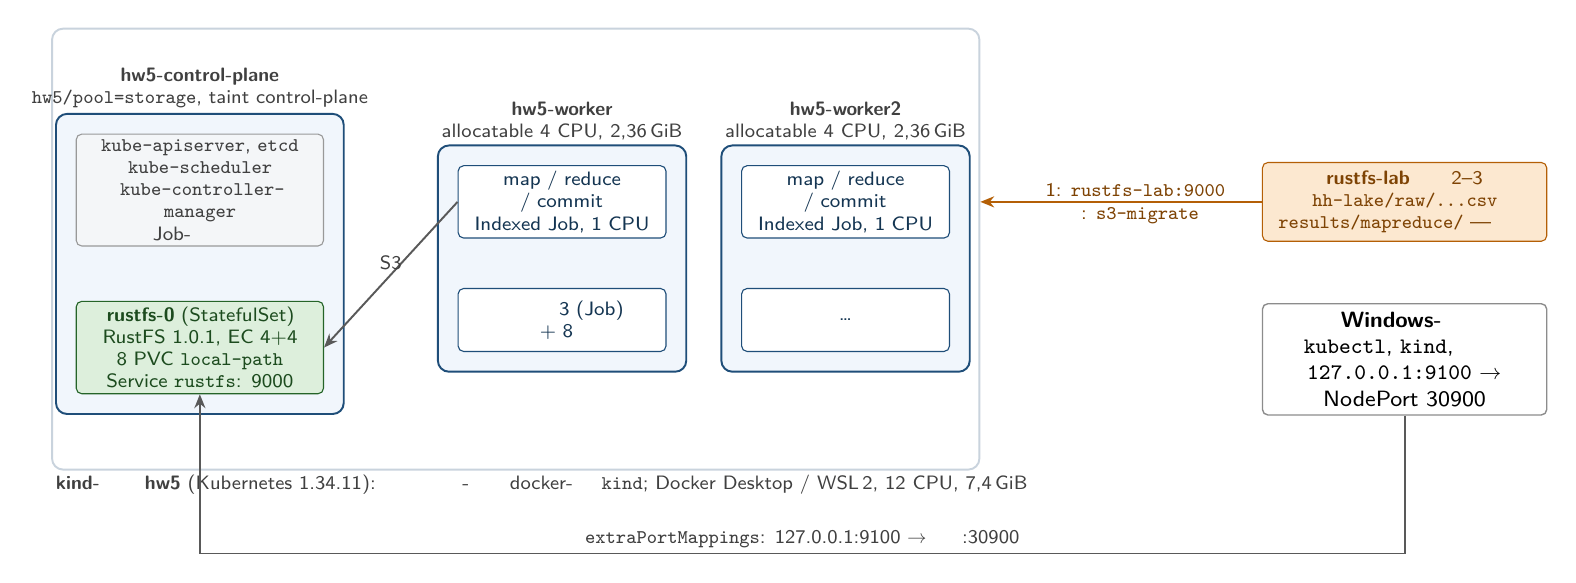
\begin{tikzpicture}[x=1cm,y=1cm]
\node[cp,text width=30mm] (api) at (0,1.15) {\mono{kube-apiserver}, \mono{etcd}\\\mono{kube-scheduler}\\\mono{kube-controller-manager}\\Job-контроллер};
\node[st,text width=30mm] (rfs) at (0,-0.85) {\tech{rustfs-0} (StatefulSet)\\RustFS 1.0.1, EC 4+4\\8 PVC \mono{local-path}\\Service \mono{rustfs}: 9000};
\node[pod,text width=25mm] (w1a) at (4.6,1.0) {map / reduce / commit\\Indexed Job, 1 CPU};
\node[pod,text width=25mm] (w1b) at (4.6,-0.5) {расчёт ДЗ 3 (Job)\\мастер + 8 воркеров};
\node[pod,text width=25mm] (w2a) at (8.2,1.0) {map / reduce / commit\\Indexed Job, 1 CPU};
\node[pod,text width=25mm] (w2b) at (8.2,-0.5) {\dots};
\begin{scope}[on background layer]
\node[zone,fill=white,fit={(api)(w2a)(0,2.9)(0,-2.1)(9.6,0)},label={[lab,anchor=north west]south west:{\textbf{kind-кластер hw5} (Kubernetes 1.34.11): три контейнера-узла в docker-сети \mono{kind}; Docker Desktop / WSL\,2, 12 CPU, 7,4\,GiB}}] (k) {};
\node[knode,fit=(api)(rfs),label={[lab,anchor=south,align=center]north:{\textbf{hw5-control-plane}\\\mono{hw5/pool=storage}, taint control-plane}}] (ncp) {};
\node[knode,fit=(w1a)(w1b),label={[lab,anchor=south,align=center]north:{\textbf{hw5-worker}\\allocatable 4 CPU, 2,36\,GiB}}] (nw1) {};
\node[knode,fit=(w2a)(w2b),label={[lab,anchor=south,align=center]north:{\textbf{hw5-worker2}\\allocatable 4 CPU, 2,36\,GiB}}] (nw2) {};
\end{scope}
\draw[arr] (w1a.west)--node[lab,above]{S3} (rfs.east);
\node[old,text width=34mm] (lab) at (15.3,1.0) {\tech{rustfs-lab} из ДЗ 2--3\\\mono{hh-lake/raw/...csv}\\\mono{results/mapreduce/} --- эталон};
\draw[arr,parC] (lab.west)--node[lab,above,text=parC!70!black]{этап 1: \mono{rustfs-lab:9000}}node[lab,below,text=parC!70!black]{перенос: \mono{s3-migrate}} (k.east|-lab.west);
\node[bx,text width=34mm] (host) at (15.3,-1.0) {\tech{Windows-хост}\\\mono{kubectl}, \mono{kind}, скрипты\\\mono{127.0.0.1:9100} $\to$ NodePort 30900};
\draw[arr] (host.south) -- ++(0,-1.75) -| node[lab,above,pos=0.25]{\mono{extraPortMappings}: 127.0.0.1:9100 $\to$ узел :30900} (rfs.south);
\end{tikzpicture}}
\end{center}}

\newcommand{\belowLimit}{512}
\newcommand{\cleanCount}{84}
\newcommand{\cleanSecs}{111}
\newcommand{\clearMax}{17}
\newcommand{\clearMin}{8}
\newcommand{\cpuMapSpan}{53}
\newcommand{\cpuMaxRun}{4}
\newcommand{\cpuPendingCount}{22}
\newcommand{\cpuPendingMax}{12}
\newcommand{\cpuPendingMean}{6{,}5}
\newcommand{\hwLimit}{704}
\newcommand{\hwLimitRaw}{661}
\newcommand{\hwThrPeriods}{48 из 364, 37 из 354, 48 из 334}
\newcommand{\hwThrottledMax}{16{,}3}
\newcommand{\hwThrottledMin}{0{,}6}
\newcommand{\imageSize}{600\,МБ}
\newcommand{\lowMapSpan}{34}
\newcommand{\lowPods}{9}
\newcommand{\lowTaskMed}{15}
\newcommand{\mapLimit}{128}
\newcommand{\mapPeakMax}{82}
\newcommand{\mapPeakMed}{79}
\newcommand{\mapPlanMed}{0{,}4}
\newcommand{\mapUploadMed}{0{,}5}
\newcommand{\measAnonMax}{534}
\newcommand{\measFileMax}{7}
\newcommand{\measPeakMax}{551}
\newcommand{\measPeakMin}{550}
\newcommand{\migSeconds}{45}
\newcommand{\migSpeed}{17{,}8}
\newcommand{\oomJemalloc}{2}
\newcommand{\oomKilled}{9}
\newcommand{\oomScoreAdj}{967}
\newcommand{\oomSeconds}{5}
\newcommand{\oomWorkers}{6}
\newcommand{\parMapSpan}{39}
\newcommand{\parMaxRun}{6}
\newcommand{\parNodeSplit}{13 и 13}
\newcommand{\parStartLag}{1{,}0}
\newcommand{\parTaskMed}{4}
\newcommand{\parTotal}{59}
\newcommand{\parWallMed}{3{,}7}
\newcommand{\preemptNode}{hw5-worker2}
\newcommand{\preemptedCount}{2}
\newcommand{\preemptedIdx}{2 и 6}
\newcommand{\preemptedRan}{10}
\newcommand{\quotaFailedCreate}{30}
\newcommand{\quotaFreeCpu}{4{,}8}
\newcommand{\quotaMapSpan}{74}
\newcommand{\quotaMaxRun}{3}
\newcommand{\quotaOverAt}{-}
\newcommand{\quotaOverCount}{0}
\newcommand{\reduceLimit}{128}
\newcommand{\reducePeakMax}{71}
\newcommand{\rfsAnonCpu}{1\,582}
\newcommand{\rfsAnonEnd}{1\,886}
\newcommand{\rfsAnonLow}{1\,726}
\newcommand{\rfsAnonPar}{1\,397}
\newcommand{\rfsAnonStart}{286}
\newcommand{\rfsGrowFirst}{556}
\newcommand{\rfsGrowLater}{122}
\newcommand{\rfsPeakEnd}{4\,004}
\newcommand{\splits}{26}
\newcommand{\tunedHeadroom}{152}
\newcommand{\tunedPeakMax}{552}
\newcommand{\tunedWallMed}{36{,}2}
\newcommand{\urgentPending}{4}
\newcommand{\urgentSpan}{26}
\newcommand{\urgentWall}{18{,}6}

\newcommand{\tabin}[1]{\csname @@input\endcsname tables/#1.tex }

\begin{document}

% ───────────────────────── ТИТУЛ ─────────────────────────
\begin{tikzpicture}[remember picture,overlay]
  \fill[accD] (current page.north west) rectangle ([yshift=-5.7cm]current page.north east);
  \fill[acc]  ([yshift=-5.7cm]current page.north west) rectangle ([yshift=-5.88cm]current page.north east);
  \node[anchor=north west,text=white,font=\sffamily\small\bfseries,inner sep=0pt] at ([xshift=1.9cm,yshift=-1.55cm]current page.north west)
     {ДОМАШНЕЕ ЗАДАНИЕ 5 \,·\, ИНЖЕНЕРИЯ ДАННЫХ \,·\, ВАРИАНТ 6};
  \node[anchor=north west,text=white,font=\sffamily\fontsize{22}{25}\selectfont\bfseries,align=left,inner sep=0pt] at ([xshift=1.9cm,yshift=-2.25cm]current page.north west)
     {Расчёт из ДЗ 3 в Kubernetes:\\пределы памяти, хранилище в кластере,\\параллельные задания и планировщик};
  \node[anchor=north west,text=white!85!accL,font=\sffamily\small,inner sep=0pt] at ([xshift=1.9cm,yshift=-5.0cm]current page.north west)
     {Васькин Виктор, J3310 \,·\, ИТМО, «Инженерия ИИ» \,·\, \mono{github.com/ViktorVaskin98/itmo-de-hw5}};
\end{tikzpicture}
\vspace*{4.9cm}

\noindent
\statcard{\hwLimit\,MiB}{предел памяти расчёта ДЗ 3: пик \measPeakMax\,MiB $\times$ 1,2; на 256Mi и \belowLimit Mi контейнер получает OOMKilled}{acc}\hfill
\statcard{0}{расхождений с ДЗ 3 по \num{100\,692} ключам у семи расчётов, топ-10 пар те же}{goodC}\hfill
\statcard{\preemptedCount\ пода}{фонового расчёта вытеснены срочным (\mono{batch-high}), их сплиты пересчитаны}{badC}\hfill
\statcard{\quotaMaxRun\ пода}{одновременно в \mono{hw5-quota} (квота 3 CPU), хотя на воркерах было свободно ещё \quotaFreeCpu\ CPU}{parC}

\vspace{6pt}
\begin{callout}[acc]{Что сделано}
Поднял kind-кластер из трёх узлов (Kubernetes 1.34.11) в Docker Desktop, собрал образ с программой из ДЗ 3 и запускал её как Job с \mono{requests} и \mono{limits}. На пределе 256Mi контейнер получил \mono{OOMKilled}. Пик памяти измерил по cgroup v2 в трёх запусках, предел \hwLimit Mi поставил по пику с запасом 20\,\% и проверил тремя запусками, а снизу пределом \belowLimit Mi (снова OOM). RustFS из ДЗ 2 перенёс в кластер (StatefulSet, восемь томов, EC 4+4), данные переложил заданием с проверкой md5. Расчёт разбил на Indexed Job: \splits\ подов map по сплитам 32\,МиБ, 4 пода reduce и задание сверки; результат совпал с ДЗ 3 по всем ключам, а частоты побайтно совпали с CSV из репозитория ДЗ 3. На этом же расчёте показал ожидание при нехватке CPU, вытеснение по \mono{PriorityClass} и квоту пространства имён. В конце сравниваю с YARN и Mesos. Все выводы команд взяты из \mono{logs/}, весь прогон запускается \mono{scripts/run\_all.ps1}.
\end{callout}

{\small\setcounter{tocdepth}{1}\tableofcontents}

\newpage
% ═════════════════════════════════════════════════════════
\section{Стенд}\label{sec:stand}

\figStand

\begin{minipage}[t]{0.49\linewidth}
\small
\textbf{Окружение.} Windows 11 Pro, Docker Desktop (Engine 29.1.2, WSL\,2), в VM 12 CPU и 7,4\,GiB, cgroup v2. Кластер поднят kind v0.33.0: каждый узел Kubernetes здесь контейнер Docker, внутри которого containerd и kubelet. \mono{kubectl} стоит из Docker Desktop, версии 1.34, поэтому и образ узлов я взял 1.34.11: клиент и сервер не должны расходиться больше чем на одну минорную версию.
\end{minipage}\hfill
\begin{minipage}[t]{0.49\linewidth}
\small
\textbf{Зачем урезан allocatable.} Все три узла видят одну и ту же VM, то есть по 12 CPU и 7,4\,GiB каждый. Без настройки планировщик считал бы, что в кластере 36 CPU, и нехватки процессора не получилось бы. Воркерам я задал \mono{system-reserved: cpu=8,memory=5Gi}: на задания остаётся по 4 CPU и 2,36\,GiB.
\end{minipage}

\term{PowerShell — kind, создание кластера, ёмкость узлов}{snippets/cluster.txt}

Сначала резерв был задан патчем \mono{KubeletConfiguration} у воркеров, но allocatable остался 12 CPU. Оказалось, что при \mono{kubeadm join} kubelet берёт общую конфигурацию из ConfigMap кластера, и такой патч у присоединяемых узлов игнорируется. Сработал флаг \mono{system-reserved} в \mono{kubeletExtraArgs} секции \mono{JoinConfiguration} (\mono{cluster/kind.yaml}). Control-plane помечен \mono{hw5/pool=storage} и закрыт taint'ом, туда попадает только хранилище, а задания идут на узлы \mono{hw5/pool=batch}.

По CPU стенд честный: 8 CPU на задания из 12 в VM. С памятью хуже. Воркеры вместе обещают 4,7\,GiB, а хранилищу на control-plane я дальше дам предел 4\,GiB (\S\,\ref{sec:rustfs-mem}), в сумме больше 7,4\,GiB, которые есть у VM. Если бы все поды одновременно дошли до своих пределов, память кончилась бы у VM целиком, и OOM пришёл бы мимо всех пределов cgroup. На моих прогонах до этого не доходило, реальные пики заметно меньше, но для настоящего кластера это был бы главный риск такой схемы.

До переноса хранилища задания читают RustFS из ДЗ 2--3 (контейнер \mono{rustfs-lab}). Я подключил его к docker-сети \mono{kind}. CoreDNS пересылает незнакомые имена в DNS Docker, поэтому из пода контейнер доступен по имени:

\term{PowerShell — старое хранилище из пода}{snippets/cluster_net.txt}

% ═════════════════════════════════════════════════════════
\section{Образ}\label{sec:image}

\codefile{Dockerfile}{../Dockerfile}

Сборка в две стадии. В первой, как в ДЗ 4, uv ставит зависимости по \mono{uv.lock} отдельным слоем, а код следующим, чтобы правка кода не пересобирала слой с pyarrow и DuckDB. Пакет \mono{hhlake} ставится в \mono{/opt/venv} обычной установкой (\mono{--no-editable}), а не ссылкой на исходники, и во вторую стадию копируется только \mono{/opt/venv}. В первом прогоне образ был одностадийным и весил 1,07\,ГБ (\mono{logs/discarded/run1/02\_image.txt}): в нём оставались сам uv и его кэш скачанных пакетов. Работает образ от пользователя с uid 10001. Расширение \mono{httpfs} для DuckDB ставится при сборке, чтобы задание сверки внутри пода не ходило за ним в интернет. Реестра у стенда нет: образ копируется в containerd узлов командой \mono{kind load}, а в манифестах стоит \mono{imagePullPolicy: Never}.

\term{PowerShell — образ и загрузка в узлы}{snippets/image.txt}

Образ весит \imageSize, примерно половина из этого окружение Python, а в нём больше всего места занимают pyarrow и библиотека DuckDB. \mono{crictl} на узле показывает меньший размер, потому что считает сжатые слои.

% ═════════════════════════════════════════════════════════
\section{Этап 1. Расчёт как задание с пределами ресурсов}\label{sec:memory}

\subsection{Манифест и как мерить память}
Программа та же, что в ДЗ 3: мастер режет объект на 26 сплитов по 32\,МиБ, пул из 8 процессов-воркеров читает их Range-запросами и считает навыки, пары и тройки, 4 редьюсера пишут part-файлы в S3. В ДЗ 3 пик я мерил через psutil по дереву процессов. Здесь важнее то, что видит ядро, ведь именно с этим числом сравнивается \mono{memory.max}. Поэтому команда пода обёрнута в \mono{hhlake.kube.memwatch}. Обёртка запускает расчёт дочерним процессом, каждые 0,1\,с читает \mono{memory.current} и \mono{memory.stat} своего cgroup, раз в 0,5\,с пишет замер в журнал, а в конце печатает \mono{memory.peak} (точный максимум, который ведёт ядро), \mono{memory.events} и \mono{cpu.stat}. Метрик-сервера (\mono{kubectl top}) в kind нет, да и он усредняет за десятки секунд, короткий пик в нём не виден.

\codefile{k8s/10-hw3-job.yaml — шаблон (\${NAME}, \${MEMORY} и др. подставляет scripts/env.ps1, готовые манифесты лежат в logs/manifests/)}{../k8s/10-hw3-job.yaml}

\mono{requests.memory} равен \mono{limits.memory}: планировщик резервирует на узле ровно столько, сколько заданию разрешено занять, и переподписки по памяти на воркере нет. По CPU запрос 2, предел 4: два ядра гарантированы, а если узел свободен, можно занять четыре. Правило \mono{podFailurePolicy} с действием \mono{FailJob} на код 137 не даёт заданию, упавшему по памяти, ещё два раза перезапуститься с тем же пределом и тем же исходом. У этого правила есть оговорка: код 137 означает любой SIGKILL, не только OOM (например, kubelet убивает так контейнер, не завершившийся за отведённое время). В этой работе других SIGKILL не было, но в общем случае проверять лучше по \mono{reason: OOMKilled}.

\subsection{Предел 256Mi: OOMKilled}
256Mi я поставил заведомо мало, чтобы увидеть, как задание останавливается по памяти. По ДЗ 3 было понятно, что этого не хватит: там всё дерево из 8 воркеров занимало около 525\,МиБ USS. Пик одного процесса был 91--97\,МиБ, но предел общий на весь контейнер.

\term{PowerShell — задание hw3-256mi}{snippets/oom.txt}

Контейнер прожил около \oomSeconds\,с. Обёртка успела записать несколько замеров, мастер распечатал план, а когда стартовали воркеры, память дошла до предела. Kubelet выставил причину \mono{OOMKilled} и код 137 (128 + SIGKILL), а Job-контроллер по правилу \mono{FailJob} сразу пометил задание \mono{Failed}. Что при этом произошло в ядре, видно в \mono{dmesg} узла:

\term{dmesg на узле — OOM внутри cgroup пода}{snippets/oom_kernel.txt}

\mono{constraint=CONSTRAINT\_MEMCG} значит, что память кончилась не у узла, а у cgroup пода (\mono{usage 262144kB, limit 262144kB}). Ядро убило не один процесс, а всю группу: kubelet ставит контейнеру \mono{memory.oom.group=1}, это видно в первой строке обёртки. Строк \mono{Killed process} \oomKilled. Это обёртка, мастер, восемь воркеров и служебный процесс \mono{resource\_tracker} из multiprocessing, который мастер запускает вместе с пулом; ещё одна строка подписана \mono{jemalloc\_bg\_thd}. Так называется фоновый поток аллокатора jemalloc, который поднимает pyarrow, и почему ядро показало его отдельной строкой, я до конца не разобрался. Для расчёта убить всю группу правильно: с одним убитым воркером мастер ждал бы до тайм-аута задачи, а с убитым мастером воркеры остались бы сиротами. \mono{oom\_score\_adj=\oomScoreAdj} kubelet считает для подов класса Burstable как $1000 - 1000\cdot\text{requests.memory}/\text{память узла} = 1000 - 1000\cdot 256\text{Mi}/7{,}36\text{Gi} \approx \oomScoreAdj$. Если память кончится уже у всего узла, ядро выберет такой процесс раньше, чем процессы Guaranteed-подов (у них $-997$).

\subsection{Замер пика}
Три запуска с пределом 2Gi, этого заведомо хватает:

\term{PowerShell — три запуска с запасом и пик по cgroup}{snippets/measure.txt}

\figplot{memory.png}{\mono{memory.current} контейнера во времени, замер раз в 0,5\,с. Пунктир показывает пределы, крест --- последний замер перед OOM-kill. Полка в начале --- мастер перед стартом пула очищает свой выходной префикс в \mono{rustfs-lab}.}{0.96}

Полке в начале графика я сначала не придал значения. По журналам подов это строка мастера \mono{cleared 0 old objects ...}: перед расчётом он просматривает и очищает свой выходной префикс, и даже пустой префикс \mono{rustfs-lab} отдавал от \clearMin\ до \clearMax\,с. Перед этапом я заранее удаляю выводы прошлых прогонов (98 объектов ушло 90\,с, около секунды на объект, это видно и в ДЗ 3), но просмотр всё равно остался медленным, кроме самого первого запуска (\mono{hw3-256mi}, 0,14\,с). От чего в RustFS зависит это время, я не выяснял. На память это не влияет, только на время запуска.

Пик от \measPeakMin\ до \measPeakMax\,MiB. Почти весь он анонимная память (до \measAnonMax\,MiB): кучи интерпретаторов и счётчики комбайнера. Это хорошо сходится с 525\,МиБ USS из ДЗ 3. Кэш файлов (\mono{file}, до \measFileMax\,MiB) появляется от временных файлов воркеров в \mono{emptyDir}. Его ядро при нехватке может выбросить, анонимную память нет: своп контейнерам kubelet не даёт.

\term{Журнал пода hw3-measure-1 (сокращено)}{snippets/measure_log.txt}

\subsection{Подбор предела}
Предел считаю от наибольшего \mono{memory.peak} трёх запусков, беру 20\,\% запаса и округляю вверх до 64\,MiB:
\[
\text{limit} = \Big\lceil \frac{\measPeakMax \cdot 1{,}2}{64} \Big\rceil \cdot 64 = \lceil \hwLimitRaw / 64 \rceil \cdot 64 = \hwLimit\ \text{MiB}.
\]
Запас нужен, потому что пик плавает. Анонимная часть почти не меняется (не больше \measAnonMax\,MiB во всех запусках), а кэш файлов зависит от того, сколько временных файлов ядро ещё не сбросило на диск. В проверочных запусках пик дошёл до \tunedPeakMax\,MiB, это на \tunedHeadroom\,MiB ниже предела. Считает всё это \mono{hhlake.kube.sizing}, а скрипт этапа подставляет результат в манифест, так что предел в \mono{logs/manifests/hw3-tuned-*.yaml} получен из журналов, а не вписан руками.

\term{PowerShell — три запуска с пределом \hwLimit Mi}{snippets/tuned.txt}

Во всех трёх \mono{memory.events: max=0}: память ни разу не упёрлась в \mono{memory.max}. Результат запуска с подобранным пределом я сверил с выводом ДЗ 3 в том же \mono{rustfs-lab}:

\term{PowerShell — hw3-tuned-1 против ДЗ 3}{snippets/tuned_verify.txt}

\subsection{Проверка снизу}
Чтобы проверить, что предел взят не с огромным запасом, запустил с \belowLimit Mi. Это чуть ниже пика анонимной памяти (\measAnonMax\,MiB): кэш файлов ядро бы отдало, а анонимную память нет.

\term{PowerShell — предел \belowLimit Mi}{snippets/below.txt}

Значит, рабочий предел лежит между \belowLimit\ (OOM) и \hwLimit\,MiB (три успешных запуска), и \hwLimit\ получен как пик плюс 20\,\%.

% ═════════════════════════════════════════════════════════
\section{Этап 2. RustFS внутри кластера}\label{sec:storage}

\subsection{StatefulSet}
Конфигурация та же, что в ДЗ 2: образ RustFS 1.0.1 с тем же digest, что у \mono{rustfs-lab} (там он был под тегом \mono{latest}), восемь папок-дисков \mono{/data/disk\{1...8\}}, erasure coding 4+4. Вместо папок на хосте восемь \mono{PersistentVolumeClaim} из \mono{volumeClaimTemplates}; провайдер \mono{local-path}, который ставит kind, создаёт под каждый том каталог на узле. Я взял StatefulSet, а не Deployment, чтобы под после перезапуска получал те же тома и то же имя \mono{rustfs-0}. Под закреплён на узле \mono{hw5/pool=storage} с допуском к taint'у control-plane и получил \mono{PriorityClass storage-critical}, так что расчёты с любым приоритетом не могут его вытеснить. Service \mono{rustfs} типа NodePort: внутри кластера это \mono{rustfs.hw5.svc.cluster.local:9000}, с хоста \mono{127.0.0.1:9100} через \mono{extraPortMappings} kind.

\term{PowerShell — хранилище в кластере}{snippets/storage.txt}

Kubernetes добавляет в под переменные окружения для каждого сервиса пространства имён. Для сервиса \mono{rustfs} это \mono{RUSTFS\_PORT=tcp://10.96.x.x:9000}, \mono{RUSTFS\_SERVICE\_HOST} и т.\,п., а это как раз префикс, по которому RustFS читает свои настройки. Чтобы они не смешивались, в манифесте стоит \mono{enableServiceLinks: false}.

\subsection{Перенос данных}
Задание \mono{s3-migrate} (\mono{hhlake.kube.migrate}) читает объекты из \mono{rustfs-lab} и пишет в RustFS кластера: сырой CSV и вывод MapReduce из ДЗ 3 (\mono{results/mapreduce} $\to$ \mono{results/hw3/mapreduce}), с которым дальше сравниваются все расчёты. md5 считается по потоку источника во время копирования, потом по повторному чтению копии, а третий раз от файла на хосте.

\term{PowerShell — перенос, контрольные суммы и раскладка по дискам}{snippets/migrate.txt}

Все три md5 совпали. ETag у копии не равен md5: объект залит multipart'ом (суффикс \mono{-51} означает число частей), а ETag такого объекта считается по частям. На каждом из восьми томов около 204\,MiB, то есть четверть от 808\,МиБ: объект разрезан на 4 блока данных и 4 блока чётности, всего вдвое больше размера, как и в ДЗ 2.

\term{PowerShell — старое хранилище больше не нужно}{snippets/storage_after.txt}

\subsection{Память самого хранилища}\label{sec:rustfs-mem}
В первом полном прогоне RustFS работал с пределом 1536Mi, который я поставил не измеряя (коммит \mono{9c77e61}). В итоге он сам получил OOMKilled посреди параллельного map, то есть ровно то, от чего этап 1 должен был уберечь. Три пода map упали с \mono{IncompleteReadError}, потому что RustFS умер, отдавая им сплит, и Job перезапустил их индексы по \mono{backoffLimitPerIndex}. Фоновый расчёт этапа 4б в том прогоне до вытеснения не дожил: все его поды получали \mono{Connection refused}. Журналы того прогона лежат в \mono{logs/discarded/run1/}.

\term{logs/discarded/run1 — RustFS и map-под во время первого прогона}{snippets/discarded.txt}

После этого я стал смотреть память RustFS по его cgroup. Анонимная память росла с каждым чтением файла и в простое не уменьшалась. Руками я пробовал выключить кэш данных объектов и кэш метаданных (\mono{RUSTFS\_OBJECT\_DATA\_CACHE\_ENABLE}, \mono{RUSTFS\_OBJECT\_CACHE\_ENABLE}), задать объём памяти явно (\mono{RUSTFS\_OVERRIDE\_MEMORY\_BYTES}) и включить возврат памяти аллокатором, но рост оставался. Эти пробы в журналы не попали, я делал их вручную. Раз у процесса, который растёт с нагрузкой, нет одного «пика», предел пришлось ставить на весь сценарий: \mono{requests} 1Gi, предел 4Gi. Старый \mono{rustfs-lab} после переноса останавливается, чтобы VM хватило памяти. В конце каждого этапа скрипт записывает память хранилища:

\term{PowerShell — память rustfs-0 после этапов 2, 3, 4а, 4б, 4в}{snippets/storage_memory.txt}

По журналу рост неравномерный. На первых двух полных чтениях (пробный прогон и \mono{par}) анонимная память выросла в среднем на \rfsGrowFirst\,MiB за чтение, на следующих четырёх уже примерно на \rfsGrowLater\,MiB, за весь прогон с \rfsAnonStart\ до \rfsAnonEnd\,MiB. Похоже, что она к чему-то стремится, но проверять, к чему, на VM с 7,4\,GiB я не стал. Рестартов не было. \mono{memory.current} при этом близко к пределу, но в основном это кэш файлов дисков, который ядро отдаёт по требованию (\mono{memory.events: max=0, oom=0}). Вывод для себя: хранилищу предел надо подбирать на всём сценарии работы и потом смотреть за ним по метрикам, одного замера мало.

% ═════════════════════════════════════════════════════════
\section{Этап 3. Параллельные задачи по частям файла}\label{sec:parallel}

\subsection{Как разбит расчёт}
В ДЗ 3 мастер сам раздавал сплиты своему пулу, а здесь это делает Kubernetes. Map оформлен как Job с \mono{completionMode: Indexed} и \mono{completions = \splits}: у каждого пода есть переменная \mono{JOB\_COMPLETION\_INDEX}, и под с индексом $i$ обрабатывает сплит $i$. Список сплитов каждый под строит сам (\mono{plan\_splits} по размеру объекта и размеру сплита). Отдельный координатор не нужен, потому что план детерминирован и у всех подов один и тот же.

Общей файловой системы у подов нет, поэтому промежуточный вывод map идёт через S3. Под пишет 12 файлов партиций (\mono{k\{1,2,3\}-r\{0..3\}.pkl}) и \mono{stats.json} в \mono{shuffle/<run>/mNNNN/}, и только потом маркер \mono{\_SUCCESS}. Если под с тем же индексом запустится ещё раз (сбой, вытеснение), он увидит маркер и выйдет, а если маркера нет, просто перезапишет файлы: map детерминирован. Reduce устроен как второй Indexed Job на 4 индекса. Он проверяет, что маркеры всех \splits\ сплитов на месте, скачивает свою партицию из сплитов текущего плана и вызывает тот же \mono{run\_reduce} из ДЗ 3. Третье задание, \mono{commit}, сводит счётчики (сумма после reduce должна совпасть с числом пар, которые выдали мапперы), пишет \mono{\_job.json} и \mono{\_SUCCESS} и запускает сверку с выводом ДЗ 3 (\mono{hhlake.verify}: FULL OUTER JOIN в DuckDB по всем ключам и топ-10 пар рядом).

\codefile{k8s/30-map-job.yaml — шаблон Indexed Job для map}{../k8s/30-map-job.yaml}

\mono{backoffLimitPerIndex: 2} даёт каждому сплиту две повторные попытки независимо от остальных; обычный \mono{backoffLimit} считал бы сбои всех индексов вместе. \mono{maxFailedIndexes: 0} значит, что если хоть один сплит не посчитался, задание провалено. В \mono{podFailurePolicy} вытеснение (\mono{DisruptionTarget}) не считается сбоем, а код 137 проваливает индекс сразу, без повторов (с той же оговоркой про SIGKILL, что и на этапе 1).

\subsection{Пределы map и reduce}
Под map обрабатывает один сплит, reduce одну партицию, это совсем другая нагрузка, чем весь расчёт в одном контейнере. Пределы я подобрал тем же способом: пробный прогон с 512Mi на под и та же формула.

\term{PowerShell — пробный прогон: пик map и reduce}{snippets/probe.txt}

Пик пода map \mapPeakMax\,MiB (медиана \mapPeakMed), reduce \reducePeakMax\,MiB, пределы получились \mapLimit Mi и \reduceLimit Mi. Почти вся эта память уходит на интерпретатор Python с boto3 и pyarrow, сами данные сплита читаются потоком.

\subsection{Прогон}
\term{PowerShell — map: сколько подов идёт одновременно}{snippets/par_run.txt}

Подов по 1 CPU одновременно работает \parMaxRun, а не 8: из 4 CPU воркера 100m уже занял под \mono{kindnet} (сетевой DaemonSet kind), и на оставшиеся 3,9 CPU помещается только три пода по 1 CPU. Такие системные запросы легко не заметить, а планировщик учитывает их наравне с моими.

\figplot{gantt_par.png}{Поды прогона \mono{par}. Серое --- \mono{Pending}, светло-синее --- под уже назначен на узел и стартует контейнер, цветное --- работа. Подписи: индекс и узел.}{0.98}

\term{Журналы пода map с индексом 7 и пода reduce с индексом 0}{snippets/par_pods.txt}

\term{PowerShell — commit и сверка с ДЗ 3}{snippets/par_commit.txt}

Все три стека совпали с выводом ДЗ 3 по всем ключам, топ-10 пар совпали построчно. Но здесь сравнение идёт с копией вывода ДЗ 3 в S3, так что формально код сверяется сам с собой. Поэтому я выгрузил частоты этого прогона тем же способом, каким в ДЗ 3 делались \mono{results/stacks/*.csv}, и сравнил с файлами из репозитория ДЗ 3 побайтно:

\term{PowerShell — частоты против results/stacks из репозитория ДЗ 3}{snippets/par_csv.txt}

Map занял \parMapSpan\,с, весь конвейер от первого пода до конца сверки \parTotal\,с. Тот же расчёт одним подом из хранилища в кластере (срочный расчёт этапа 4б) отработал за \urgentWall\,с, то есть параллельная раскладка здесь медленнее. Причин несколько: у каждого пода один процессор, а в одном контейнере восемь воркеров делили четыре; каждая задача заново поднимает интерпретатор и строит план по объекту (медиана \mapPlanMed\,с); выгрузка партиций в S3 занимает ещё \mapUploadMed\,с (медиана); и через S3 идёт перемешивание, которого в одном контейнере нет. На 808\,МиБ всё это перевешивает. Зато каждый сплит теперь отдельная единица работы, которую можно поставить на любой узел, перезапустить по отдельности и вытеснить, не трогая остальные, и это используется дальше.

% ═════════════════════════════════════════════════════════
\section{Этап 4. Планировщик: процессор, приоритеты, квота}\label{sec:sched}

\subsection{Ожидание при нехватке процессора}
Тот же map, но каждый под просит 1500m CPU. На воркер помещается два таких пода (3 CPU из 3,9 свободных), а третьему уже не хватает:

\term{PowerShell — поды Pending и сообщение планировщика}{snippets/cpu.txt}

В сообщении планировщика из трёх узлов один отброшен из-за taint'а (это control-plane), у двух \mono{Insufficient cpu}. Дальше про вытеснение: на control-plane оно не поможет (\mono{Preemption is not helpful}), а на воркерах некого вытеснять (\mono{No preemption victims found}), потому что все поды одного приоритета. На каждом воркере при этом простаивают 0,9 CPU, которые ни одному поду не подходят, это фрагментация. Ожидающие поды стоят в очереди планировщика и пробуются снова, когда на узле что-то освобождается.

\figplot{gantt_cpu.png}{Поды прогона \mono{cpu}: одновременно работает \cpuMaxRun, остальные ждут в \mono{Pending}.}{0.98}

\term{PowerShell — сводка ожидания}{snippets/cpu_after.txt}

В \mono{Pending} дольше секунды ждали \cpuPendingCount\ подов из \splits, дольше всех \cpuPendingMax\,с. Map занял \cpuMapSpan\,с против \parMapSpan\,с у прогона по 1 CPU. Последняя строка показывает другой вид ожидания из-за процессора, уже внутри работающего контейнера. У расчёта из ДЗ 3 с \mono{cpu.max = 4 CPU} квота CFS кончалась в \hwThrPeriods\ периодов по 100\,мс (три запуска с подобранным пределом), и до конца такого периода процесс ждал. \mono{throttled} в секундах здесь суммируется по всем процессорам, поэтому он не равен времени простоя по часам и показателен меньше, чем доля периодов. В \mono{Pending} под ждёт решения планировщика, а здесь он уже запущен и ждёт своей доли процессора.

\subsection{Вытеснение задачи с низким приоритетом}
Классы приоритета: \mono{batch-low} (1000) для фоновых расчётов, \mono{batch-high} (100000) для срочных и \mono{storage-critical} для хранилища. Фоновый расчёт \mono{low} --- это map со сплитами по 128\,МиБ (7 задач по \lowTaskMed\,с, чтобы они не успевали закончиться сами) по 1 CPU; шесть задач занимают все места на воркерах, седьмая ждёт. Срочный расчёт --- программа из ДЗ 3 с тем же манифестом, что на этапе 1, подобранным пределом \hwLimit Mi и запросом 2 CPU, но с классом \mono{batch-high} и хранилищем уже в кластере.

\term{PowerShell — срочный расчёт приходит в занятый кластер}{snippets/preempt.txt}

Планировщик не нашёл узла, куда срочный под помещается, и стал выбирать, кого снять. На \mono{\preemptNode} свободно 0,9 CPU, одного вытесненного пода (1 CPU) мало, двух хватает. Обоим он поставил условие \mono{DisruptionTarget} с причиной \mono{PreemptionByScheduler} и удалил их. Срочный под получил узел через \urgentPending\,с после создания. Вытесненные поды (индексы \preemptedIdx) успели проработать около \preemptedRan\,с.

Здесь была ошибка, которую я нашёл при отладке. Сначала вытесненные поды не останавливались: они дорабатывали свой сплит, и Job засчитывал их как успешные. Дело оказалось в том, что PID 1 в контейнере моя обёртка \mono{memwatch}, а процесс с PID 1 без своего обработчика SIGTERM игнорирует. Kubelet посылает SIGTERM и ждёт \mono{terminationGracePeriodSeconds} (30\,с), прежде чем убить, а короткая задача за это время успевала закончиться. Журнала того прогона у меня не осталось, вытесненные поды удаляются вместе с логами; после этого скрипт стал сохранять их журналы. Теперь обёртка пересылает сигнал расчёту и выходит с кодом 143:

\term{Журнал вытесненного пода}{snippets/preempt_victim.txt}

\figplot{gantt_preempt.png}{Фоновый и срочный расчёты. Красные поды вытеснены, их индексы (\preemptedIdx) созданы заново и досчитаны позже.}{0.98}

\term{PowerShell — оба расчёта закончились и совпали с ДЗ 3}{snippets/preempt_after.txt}

У \mono{low-map} поле \mono{FAILED} пустое: благодаря правилу \mono{Ignore} для \mono{DisruptionTarget} вытеснение не считается неудачей и не тратит попытки \mono{backoffLimitPerIndex}. Подов \lowPods\ на 7 индексов, лишние как раз пересозданные. Оба расчёта совпали с ДЗ 3.

\subsection{Квота пространства имён}
Пространство \mono{hw5-quota} получило квоту: 3 CPU и 1Gi на \mono{requests} и на \mono{limits}, 10 подов, 4 задания. Квота на \mono{cpu} и \mono{memory} обязывает каждый под указывать эти поля, и под без них при создании отклоняется, пока нет \mono{LimitRange} со значениями по умолчанию.

\term{PowerShell — квота, под без ресурсов и LimitRange}{snippets/quota_admission.txt}

Тот же map (по 1 CPU, \mono{parallelism: 8}) в этом пространстве:

\term{PowerShell — квота во время прогона}{snippets/quota_run.txt}

Отличие от нехватки CPU в том, где задача ждёт. Там поды создавались и стояли в \mono{Pending}, и решение было за планировщиком. Здесь лишние поды вообще не создаются: admission-контроллер квоты отклоняет запрос Job-контроллера (\mono{FailedCreate ... exceeded quota}), и тот пробует снова при следующей синхронизации, за прогон \quotaFailedCreate\ отказов. Одновременно работало \quotaMaxRun\ пода, хотя на двух воркерах вместе (по \mono{Allocated resources} выше) оставалось свободно ещё \quotaFreeCpu\ CPU. Квота ограничивает пространство имён и про свободные ресурсы кластера ничего не знает.

\figplot{gantt_quota.png}{Поды map в \mono{hw5-quota} идут по три, \mono{Pending} нет: остальные поды ещё не созданы.}{0.98}

\term{PowerShell — итог в hw5-quota}{snippets/quota_after.txt}

% ═════════════════════════════════════════════════════════
\section{YARN, Mesos и Kubernetes}\label{sec:yarn}
\subsection{Что чему соответствует}

Во всех трёх системах роли примерно одни и те же: кто-то ведёт учёт ресурсов на узлах, кто-то решает, куда поставить задачу, агент на узле запускает процесс и следит за ним, и кто-то знает логику самого приложения (какие задачи, в каком порядке, что делать при отказе). Отличаются системы тем, кому какая роль достаётся.

\tabin{mapping}

Больше всего на моих прогонах ощущалась разница в последней роли. В YARN у приложения MapReduce есть свой ApplicationMaster. Он знает про фазы map и reduce, сам запрашивает контейнеры у ResourceManager, перезапускает упавшие задачи и запускает reduce, когда закончился map. В Kubernetes такого слоя нет. Job-контроллер держит нужное число успешных подов и перезапускает упавшие индексы, но про то, что reduce можно начинать только после всех map, он не знает. У меня эту работу делает скрипт \mono{scripts/05\_parallel.ps1}: ждёт \mono{par-map}, отправляет \mono{par-reduce}, потом \mono{par-commit}. В настоящих системах для этого ставят Argo Workflows, оператор Spark или Kubeflow, то есть надстройки. В Mesos ещё дальше: сам Mesos задачи не размещает, а только предлагает ресурсы, и размещение, и порядок пишет фреймворк.

\subsection{Кто решает, где запустить задачу}

\textbf{YARN.} Планировщик один, он в ResourceManager. ApplicationMaster присылает запросы вида «$N$ контейнеров по $X$\,МБ и $Y$ vcores, лучше на таком-то узле или стойке». Планировщик (Capacity или Fair) выдаёт контейнеры по мере освобождения ресурсов; о свободных ресурсах он узнаёт из пульса NodeManager. Место выбирает RM, но с учётом пожеланий приложения о локальности данных.

\textbf{Mesos.} Планирование двухуровневое. Мастер не знает, что нужно задачам. Его аллокатор (DRF, Dominant Resource Fairness между ролями) \emph{предлагает} фреймворку ресурсы конкретного агента, а планировщик фреймворка решает, взять их и что на них запустить или отказаться. Выбор места целиком на фреймворке, зато мастер простой.

\textbf{Kubernetes.} Планировщик тоже один (\mono{kube-scheduler}), и о приложении он ничего не знает. Он берёт поды из очереди по одному (очередь отсортирована по приоритету), отбрасывает узлы, куда под не помещается (\mono{requests} против \mono{allocatable}, \mono{nodeSelector}, taints), оценивает оставшиеся и записывает \mono{nodeName}. В моих манифестах это видно напрямую: поды map с \mono{nodeSelector: hw5/pool=batch} попадали только на два воркера, а RustFS с допуском к taint'у control-plane --- только на \mono{hw5-control-plane}. Индексы map планировщик разложил по воркерам примерно поровну (\parNodeSplit\ подов), хотя о сплитах ничего не знает.

\subsection{Как задаются ресурсы и что бывает при превышении}

\textbf{YARN.} У контейнера один размер: сколько памяти и vcores запросило приложение, с округлением вверх до кратного \mono{yarn.scheduler.minimum-allocation-mb} (по умолчанию 1024\,МБ). Отдельно «гарантии» и «потолка» нет. Память проверяет NodeManager: монитор контейнеров раз в несколько секунд складывает RSS всего дерева процессов и, если сумма больше выделенного, убивает контейнер с сообщением \mono{is running beyond physical memory limits}. Есть и проверка виртуальной памяти (\mono{vmem-pmem-ratio}), на которой контейнеры чаще всего и падают. Строгий предел через cgroups тоже можно включить. Процессор в Capacity Scheduler по умолчанию вообще не учитывается: \mono{DefaultResourceCalculator} смотрит только на память, vcores начинают учитываться с \mono{DominantResourceCalculator}, а жёстко ограничиваются только через cgroups.

\textbf{Kubernetes.} Величин две: \mono{requests} учитывает планировщик (сколько «занято» на узле), \mono{limits} kubelet записывает в cgroup контейнера (\mono{memory.max}, \mono{cpu.max}). Память проверяет не kubelet по таймеру, а ядро в момент выделения страницы, поэтому OOM наступает сразу и «проскочить» между замерами нельзя. В моём запуске с пределом 256Mi контейнер прожил около \oomSeconds\,с: ядро сначала выбросило кэш файлов, потом освобождать стало нечего, и оно вызвало OOM-killer внутри cgroup пода. Kubelet ставит \mono{memory.oom.group=1}, поэтому были убиты все процессы контейнера. В YARN при превышении тоже убивается весь контейнер, так что смысл одинаковый, а механизмы разные: опрос RSS по таймеру против проверки в ядре. Процессор Kubernetes ограничивает квотой CFS. У расчёта из ДЗ 3 с \mono{cpu.max} в 4 CPU квота кончалась в \hwThrPeriods\ периодов по 100\,мс: в этих периодах процесс ждал следующего, уже будучи запущенным.

\textbf{Mesos.} Ресурсы приходят в предложениях (\mono{cpus}, \mono{mem}, \mono{disk}, порты). Задача забирает часть предложения, а изоляцию на агенте делает containerizer через те же cgroups.

\subsection{Что происходит, когда ресурсов не хватает}

В \textbf{YARN} запросы контейнеров от ApplicationMaster просто остаются невыполненными: приложение в состоянии \mono{RUNNING}, часть задач ждёт. Если в очереди нет места даже под сам ApplicationMaster, приложение ждёт в состоянии \mono{ACCEPTED}. В \textbf{Mesos} фреймворк не получает подходящих предложений (или отказывается от неподходящих) и ждёт. В \textbf{Kubernetes} под создаётся сразу и висит в \mono{Pending} с событием \mono{FailedScheduling}. В моём прогоне с 1500m CPU на под планировщик написал \mono{Insufficient cpu} для обоих воркеров, хотя на каждом оставалось по 0,9 CPU: два пода по 1,5 CPU занимают 3 из 3,9, третий не помещается. Это обычная фрагментация при упаковке: в YARN она тоже есть и даже крупнее, потому что vcores там целые, а память округляется до \mono{minimum-allocation-mb}. Дольше всех под ждал \cpuPendingMax\,с, а map в целом шёл \cpuMapSpan\,с вместо \parMapSpan.

\subsection{Приоритеты и вытеснение}

В \textbf{YARN} (Capacity Scheduler) вытеснение в первую очередь работает между очередями. Если очередь заняла больше гарантированной доли, а другой очереди её доля нужна, монитор вытеснения снимает контейнеры у той, что взяла лишнее. В Hadoop 3 есть и вытеснение внутри очереди по приоритету приложений (\mono{intra-queue-preemption}).

В \textbf{Mesos} общего вытеснения между фреймворками нет. Мастер может перестать предлагать ресурсы или попросить их вернуть (inverse offers, для обслуживания узлов). Есть revocable-ресурсы: выделенные, но фактически не используемые ресурсы, которые раздаются повторно (переподписка) и которые можно отобрать. Что именно остановить, решает фреймворк. Проект при этом почти не развивается: последний релиз 1.11.0 вышел в 2020 году.

В \textbf{Kubernetes} вытеснение идёт по приоритету пода. Если под с высоким \mono{PriorityClass} никуда не помещается, планировщик ищет узел, где удаление подов с меньшим приоритетом освободит место, записывает поду \mono{nominatedNodeName} и удаляет выбранные поды. В моём прогоне срочный расчёт (\mono{batch-high}, 2 CPU) пришёл, когда поды \mono{batch-low} занимали на воркерах все места. Планировщик снял \preemptedCount\ пода на одном узле, и они получили условие \mono{DisruptionTarget} с причиной \mono{PreemptionByScheduler}. Чтобы фоновое задание из-за этого не упало, в манифесте map есть правило \mono{podFailurePolicy} с действием \mono{Ignore} для \mono{DisruptionTarget}. Вытесненные индексы создаются заново и не тратят \mono{backoffLimitPerIndex}. Фоновый расчёт закончился позже, но с тем же результатом, что в ДЗ 3. Повторно считать вытесненный сплит безопасно: map пишет вывод сплита в S3 целиком и только потом ставит \mono{\_SUCCESS}.

\subsection{Квоты}

Очередь Capacity Scheduler в \textbf{YARN} --- это доля кластера с гарантией (\mono{capacity}) и потолком (\mono{maximum-capacity}). Пока другие очереди простаивают, очередь может занять больше гарантии, а когда ресурсы нужны другим, её поджимают вытеснением. В \textbf{Mesos} похожую роль играют роли с весами (доля в DRF), квотами и резервированиями ресурсов на агентах.

\textbf{ResourceQuota} в Kubernetes устроена иначе. Это жёсткий потолок на сумму \mono{requests} и \mono{limits} в пространстве имён, и проверяется он при \emph{создании} пода, а не при планировании. Поэтому в \mono{hw5-quota} лишние поды map не висели в \mono{Pending}: их просто не удавалось создать. Job-контроллер получал \mono{FailedCreate: exceeded quota} и пробовал снова при следующей синхронизации, и поды шли волнами по три, по мере того как заканчивались предыдущие, хотя на воркерах оставалось свободно ещё \quotaFreeCpu\ CPU: занять их квота не даёт. Гарантии, как в YARN, она тоже не даёт: если чужие поды займут кластер, мои будут ждать при неиспользованной квоте. Очереди с заимствованием и справедливым делением в Kubernetes добавляют надстройки: Kueue (\mono{ClusterQueue} и cohort), Volcano, YuniKorn (последний прямо переносит модель очередей YARN). Ещё одно отличие: квота на \mono{cpu} и \mono{memory} требует, чтобы эти поля были у каждого пода. Под без них отклоняется, пока нет \mono{LimitRange} со значениями по умолчанию; в YARN такой проблемы нет, там всегда есть минимальный размер контейнера.

\subsection{Что когда выбирать}

YARN рассчитан на пакетную аналитику вокруг HDFS: локальность данных, очереди с долями между командами, готовые ApplicationMaster для MapReduce, Spark и Tez. Mesos --- тонкий слой распределения ресурсов, поверх которого каждый фреймворк пишет свой планировщик, гибко, но всё приходится делать самому. Kubernetes держит описанное состояние подов и одинаково подходит и для сервисов, и для заданий, а пакетные вещи (стадии, очереди с заимствованием, gang scheduling) приходят надстройками. В моей задаче данные лежат в S3, а не в HDFS, так что главное преимущество YARN, локальность, здесь не работает. Kubernetes дал всё, что требовалось: пределы памяти с OOM в ядре, параллельное задание по индексам, приоритеты и квоты. Связку стадий map $\to$ reduce пришлось делать скриптом.


% ═════════════════════════════════════════════════════════
\section{Выводы}\label{sec:conclusions}

\begin{itemize}
\item Предел памяти считается на весь контейнер, а не на процесс. Все процессы контейнера вместе дали пик \measPeakMax\,MiB, и 256Mi кончились через \oomSeconds\,с. По \mono{memory.peak} в трёх запусках и запасу 20\,\% вышло \hwLimit Mi. \belowLimit Mi уже даёт OOM, потому что это ниже пика анонимной памяти, которую ядро отдать не может.
\item OOM в Kubernetes проверяет ядро в момент выделения памяти, а kubelet ставит \mono{memory.oom.group}, поэтому убивается весь контейнер. В манифесте стоит учесть \mono{podFailurePolicy}, чтобы не повторять задание с тем же пределом.
\item Хранилище в кластере подчиняется тем же пределам. RustFS с пределом, поставленным наугад, упал по OOM посреди расчёта, а его память растёт с прочитанным объёмом, так что предел для него надо подбирать по всему сценарию.
\item Indexed Job хорошо ложится на MapReduce: индекс равен номеру сплита, повторы идут по индексу, обмен через S3 с маркером готовности. Семь расчётов в кластере (этап 1 с подобранным пределом, пробный, \mono{par}, с нехваткой CPU, фоновый после вытеснения, срочный, в квоте) совпали с ДЗ 3 по всем \num{100\,692} ключам, а частоты \mono{par} побайтно совпали с CSV из репозитория ДЗ 3. На файле в 808\,МиБ параллельная раскладка медленнее одного пода, выигрыш у неё в отказоустойчивости и гибкости размещения. Связки стадий в Kubernetes нет, её делает скрипт.
\item На планировщик влияют мелочи, которые легко пропустить: 100m сетевого DaemonSet'а уменьшили число параллельных подов с 8 до 6, запрос 1500m оставлял на каждом узле по 0,9 CPU, а PID 1 без обработчика сигналов не давал вытеснению остановить задачу.
\item Квота и нехватка ресурсов выглядят похоже, задача ждёт в обоих случаях, но устроены они по-разному: квота не даёт создать под даже при свободном кластере, а при нехватке под создан и стоит в \mono{Pending}, пока не освободится узел.
\end{itemize}

\end{document}
